\documentclass[12pt,a4paper]{article}
\linespread{1}
\usepackage[utf8]{inputenc}
\usepackage[margin=1in]{geometry}
\usepackage{amsmath}
\usepackage{amsthm}
\usepackage{amsfonts}
\usepackage{wrapfig,lipsum,booktabs}
\usepackage{ragged2e}
\usepackage{amssymb}
\usepackage[font=footnotesize,labelfont=bf]{caption}
\usepackage{subcaption}
\usepackage[usenames, dvipsnames]{color}
\usepackage{graphicx}
\usepackage{float}
\usepackage{hhline}
\usepackage{tabularx}
\usepackage[citestyle=authoryear, bibstyle=authoryear,backend=biber]{biblatex}
\DeclareUnicodeCharacter{8208}{-}

\newtheorem{theorem}{Theorem}

\newcommand{\rojo}{\textcolor{red}}
\newcommand{\azul}{\textcolor{blue}}

\bibliography{ref.bib}
\title{Outlining a Posterior-Approximating HMCMC Algorithm}

\begin{document}
\maketitle
\section{Brief Intro}
We would like to design an MCMC algorithm that combines Hamiltonian MCMC (HMCMC) \rojo{(why didn't I use HMC instead)} \parencite{neal_mcmc_2012,betancourt_geometric_2014,betancourt_conceptual_2017} and the approximate posterior + refinement approach of the Shrinking Bullseye \parencite{conrad_accelerating_2015}.  This will hopefully allow basically a fast and flexible ``black box'' tool for fast simulation-based inference with some arbitary mathematical model; looking specifically for usage with ODE models from ecology but ideally this could be handy for any general application of simulation-oriented Bayesian stats.

The basic skeleton of an HMCMC algorithm procedes as follows:
\begin{enumerate}
\item Consider the sampler at point $\vec{q}_n$ in parameter space with posterior density $\pi(\vec{q} | \vec{y})$ where $\vec{y}$ is the observed data (supressed going forward) .
\item Draw a momentum vector $\vec{p}_n$ from the distribution $\pi(\vec{p} | \vec{q} ) = \text{N}(\vec{p} |0, M)$ where $M$ is the mass matrix (in vanilla HMCMC this is usually chosen to be the covariance matrix of $\pi(\vec{q}|\vec{y})$ but for Riemanian HMCMC I believe one uses the Hessian of $\pi(\vec{q})$ with respect to $\vec{q}$ evaluated at $\vec{q}_n$, or something similar).
\item We then numerically integrate the following Hamiltonian with step size $h$ for $s$ steps (the integration time $sh$ is a free parameter for the sampler, and needs to be chosen wisely based on the geometry of the posterior), with initial conditions $(\vec{q}_n, \vec{p}_n)$:
\begin{equation}
\begin{split}
\dot{\vec{q}} &= M^{-1} \vec{p} \\
\dot{\vec{p}} &= - \nabla ln(\pi(\vec{q}))\\
\end{split}
\end{equation}
\item This integration is typically done by the leapfrog method (see Appendix), but any other \textit{symplectic} numerical integrator will work.
\item After integrating to time $sh$ the candidate points $q_{n+1}, p_{n+1}$ (supressing vector notation) are set as $q_{n+sh}, p_{n+sh}$.  To make the process reversible we need to now negate $p_{n+1}$, so our candidate points are $q_{n+1}, -p_{n+1}$.  Then the candidate $q_{n+1}$ gets plugged into the usual Metropolis accept/reject probability.  Doing a Metropolis accept/reject would not be necessary if we could integrate (1) without error, but due to the error in (2) we would get biased estimates without the Metropolis step.
\end{enumerate}

\section{Testing Approximation Methods}
Based on some squishy problem considerations (see Appendix) and conversation with Dr. Ian Grooms (see update from 6/2) I identified two approximating algorithms to compare: (1) Local Quadratic Regression (LQR) and (2) radial basis functions (specifically Thin Plate Splines, TPS).  These are both gridless methods, so are well-suited to ad hoc additions to the approximating set $S$.  For a first look-over I implement both and compare their performance (the TPS was implemented with no low-rank approximation, as it reduced approximation quality substantially without providing a substantial computational speedup).

For comparison of performance I used the test density function:
\begin{equation}
\pi(x,y) = \text{Exp} \left( -P*(A*x^2*y^2 + x^2 + y^2 - B*x*y - C*x - C*y) \right)
\end{equation}
With $A = C = 1$, $ B =10$ and $ P = 0.05$ (Fig. 1).  For gradient calculations I used the NumPy \texttt{gradient()} function, which computes the gradient by central differences.  It should be noted that for both LQR and TPS one should be able to compute the gradient by hand, and I initially had done so, but it was simpler in implementation to just use central differences for now.  To compare the methods I fit them with 300 points chosen uniformly over the square $[-15,15] \times [-15,15]$ and computed the gradient at 1e5 gridpoints over the square $[-6,6] \times [-6,6]$.  Letting $\hat{\pi}_i$ denote the approximation from method $i$, I computed the max gradient error as:
\[
\epsilon_i = \frac{ \text{max}_{j} \left( \Vert \nabla \hat{\pi}_i(\vec{x}^{(j)}) - \nabla \pi(\vec{x}^{(j)})  \Vert \right) } { \text{max}_j \left( \Vert \nabla \pi(\vec{x}^{(j)}) \Vert \right) }
\]
Where the max's are taken over the grid points $\vec{x}^{(j)}$. I similarly computing a max function error:
\[
e_i = \frac{ \text{max}_{j} \left( \Vert \hat{\pi}_i(\vec{x}^{(j)}) - \pi(\vec{x}^{(j)})  \Vert \right) } { \text{max}_j \left( \Vert \pi(\vec{x}^{(j)}) \Vert \right) }
\]

The thin plate splines fared substantially better, with $e_{\text{TPS}} = 0.319$ and $\epsilon_{\text{TPS}} = 0.826$ compared to $e_{\text{LQR}} = 0.596$ and $\epsilon_{LQR} = 57.9$.  This was calculated with a TPS smoothness parameter $\lambda = 1e-7$.  To asses how varying this parameter changed the TPS fit I re-computed $e_{\text{TPS}}$ and $\epsilon_{\text{TPS}}$ for each $\lambda \in [1e-10, 1e-7,1e-4, 1e-1, 1, 10, 100]$.  Virtually no effect of varying $\lambda$ was detected on either measure of error, however, all values of $\lambda$ $e_\text{TPS} = 1.105$ and $\epsilon_\text{TPS} = 0.826$ with any differences being on the order of $1e-6$.

\begin{figure}
\centering
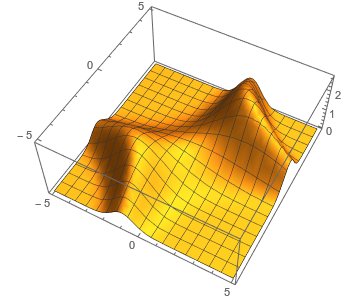
\includegraphics[scale=.6]{./Figs/test_dense.png}
\caption{The test density function in (3) with $A = 1, B =10, C = 1, P = 0.05$}
\end{figure}

I also tested how the gradient error might effect Hamiltonian dynamics when numerically integrated with leapfrog.  I chose a random initial, 2D position and momentum vector uniformly from the square $[-6,6] \times [-6,6]$, and then integrated forward for a random number of steps from 10 to 100, with fixed step size $h = 1e-5$.  I repeated this for 100 such initial conditions with the test density, as well as the LQR and TPS approximated densities.  I calculated the path error for method $i$ as $\rho_i = \frac{ \sum\limits_s \Vert q_i^{(s)} - q^{(s)} \Vert }{ \sum\limits_s \Vert q^{(s)} - q^{(s-1)} \Vert }$, $q_i^{(s)}$ is the $s^{\text{th}}$ leapfrog step for $V(x)$ approximated by method $i$, and $q^{(s)}$ is same for the ``true'' $V(x)$.  This is effectively the path integral of the leapfrog error normalized by the arc length of the true s-step forward integration.  Normalizing by arc length doesn't give a sense of how the error might behave in the long-time, but intuitively one expects the error to behave fairly poorly in the long time anyways so I wasn't as interested in measuring it.  My hope here is to instead get a sense of how badly the approximated potentials effect the Hamiltonian dynamics ``on average''; if both methods behave similarly on average I may then dig into the long-time error to see if there's an important difference there.

Averaging over the random initial conditions and step sizes we get $E[\rho_\text{LQR}] = 1.09$ and $\text{Var}[\rho_\text{LQR}] = 0.193$, while for TPS we get $E[\rho_\text{TPS}] = 0.372$ and $\text{Var}[\rho_\text{TPS}] = 0.398$.  The high variance of the TPS path error was surprising to me, although looking at the histograms of the observed error (Fig. 2) we see that the TPS approximated potential does generally perform better than the LQR approximation.  It does, however, appear that both methods had a small number of equally bad initial conditions or step sizes resulting in atypically large error.  I'm guessing that these were a particularly sensistive IC or chaotic region for the Hamiltonians.

\begin{figure}
\centering
\begin{tabular}{cc}
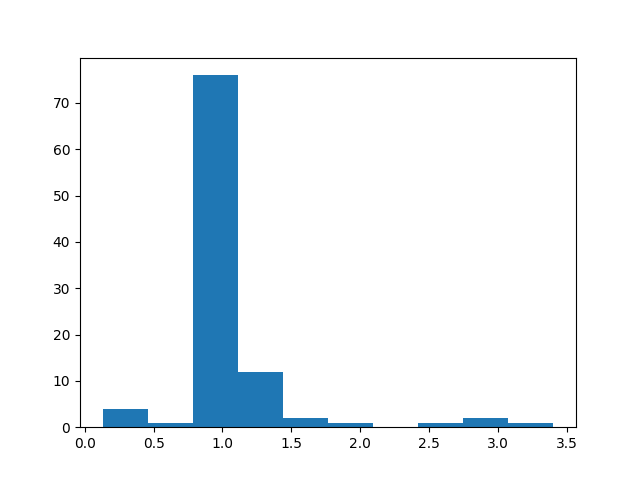
\includegraphics[scale=.5]{./Figs/lqr_ham_hist.png} & 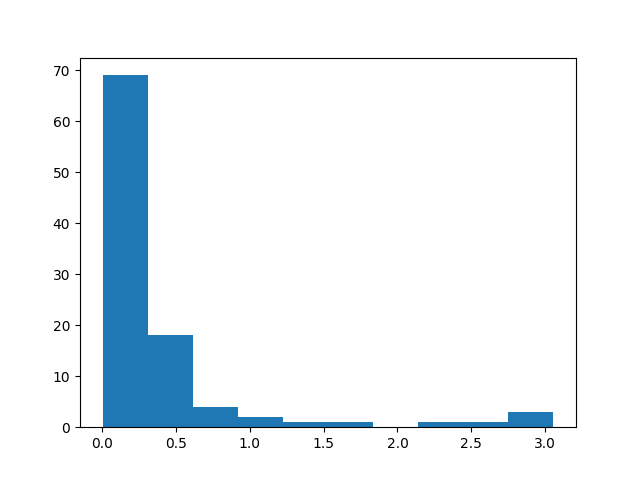
\includegraphics[scale=.5]{./Figs/tps_ham_hist.png}\\
(a) & (b)\\
\end{tabular}
\caption{Histogram of path errors for (a) the LQR approximated potential and (b) the TPS approximated potential}
\end{figure}

\section{Outline of Posterior Approximating HMCMC}
Based on these results I decided to go ahead with drafting a Hamiltonian MCMC sampler using the TPS approximated posterior.  Currently the rough stages of this algorithm are very similar to the Shrinking Bullseye:
\begin{enumerate}
\item \textit{Initialize:}
\begin{enumerate}
\item Drum-up some good set of interpolating points $S$, calculate and $f(S) = {P(s) : s \in S}$ for a posterior density $P$ from data $\vec{y}$ over parameter vector $q$, using $q$ to reflect that this is also the generalized position vector.  It's better to interpolate $P$ with $\hat{P}$ and then use $\hat{V}(q) = - ln(|\hat{P}(q)|)$ as interpolating $V$ itself might give a potential energy function with undesirable characteristics, e.g. decaying to 0 at infinity.
\item Following Wendland here (2007, ``Computational Aspects of Radial Basis Function Approximation''). Let $\psi(r)$ be our radial basis function (in this application it's the thin plate spline function, in $\mathbf{R}^2$ this is $\psi(r) = r^2 \text{ln}(r)$, but in higher dimensions the definition gets \textit{wonky} and I'm not going to typeset all that) and $\Pi_{m,d}(x)$ be the matrix of multivariate  monomials of degree $\leq m$ in $d$ variables.  These monomials are, AFAIK, basically a regularization term; when you take the first $m$ derivatives in whatever smoothness penalty you're using you kill off any polynomial terms so we need to add them back in to make the space of interpolate-able functions sufficiently large or something similar; alternately it guarantees that the interpolation matrix will always be invertible which is nice, although I think you could just replace the inverse with the least-squares solution and then drop the polynomials altogether.  Construct the interpolation matrix:
\[
C =  \left[ 
\begin{array}{cc}
\Psi & \Pi_{m,d}\\
\Pi_{m,d} & 0_{m+n}\\
\end{array}
\right]
\]
Where $\Psi = [\psi(\Vert s_i - s_j \Vert)]_{i,j}$, where the $s_i$ are the $n$ interpolating points in $S$.  We then want to solve the matrix equation:
\begin{equation}
C \gamma_n = \left[ \begin{array}{c} f(S)\\ 0\\ \end{array} \right] = y_n
\end{equation}

So our coefficient vector is $\gamma_n = C^{-1} y_n$.

\item Now pick a starting point $q_0$ and finish the initialization stage.

\end{enumerate}

\item \textit{Sample}
\begin{enumerate}
\item Let the sampler be at parameter position $q$.  Propose a point $q'$ by numerically integrating a Hamiltonian system on the approximated potential energy surface $\hat{V}(q)$ with a random initial momentum $p \sim N(0, M)$ and quadratic kinetic energy (ie. $K(p) = p^T M P$ where $M$ is a user-chosen mass matrix.  For vanilla HMCMC this is optimally set to the covariance matrix in $q$; in Riemannian HMCMC this is the Hessian of $V(q)$.
\item Check if $S$ requires refinements:
\begin{enumerate}
\item Pool the $N$ nearest points to the numerical path from Step 1.  That is, let $q^{i}$ be the $i^{\text{th}}$ step in the proposal trajectory where $i = 1,...,s$ and $q_1 = q$, our current sample.  Then set $B_N(q^{(i)})$ as its $N$ nearest neighbors and take $B = \bigcup\limits_{i=1}^{s}B_N(q^{i})$.
\item Now perform some kind of cross validation on the proposal process using the same momentum $p$.  Let $\hat{V}_k$ be the RBF interpolated potential calculated using the interpolating set $S_k = S/B \cup B_k$ where $B_k$ is a random subset $B_k \subset B$ for $k =1,...,K$.  Starting from $(q,p)$ run the leapfrog integrator to get new candidates $q_k'$.  Evaluate the acceptance probability $\alpha(q,q_k')$ for each CV candidate, if $\text{max}_k \alpha(q, q_k') - \text{min}_k \alpha(q, q_k') > \epsilon$ where $\epsilon$ is some preset tolerance then we add points to $S$ following some optimality criteria and repeat from (i).  If $\text{max}_k \alpha(x, x_k') - \text{min}_k \alpha(x, x_k') < \epsilon$ then we add no refinements and proceed to (c) below.
\end{enumerate}
\item  Accept $q'$ with probability $\alpha(q,q')$, otherwise stay at $q$.  Go to (a).
\end{enumerate}
\end{enumerate}

One could resolve the equation in (3) during every CV iteration in (ii), however it is computationally cheaper to use rank-one updates and then just perform leave one out CV for a handful of points in $B$.  So let's go through what those will look like.

\section{Rank One Updates for Radial Basis Functions}
First we should note that $\Psi$ and hence $C$ are symmetric, and furthermore $C$ is invertible.  We need to perform two operations on the interpolation matrix $C$: row/column additions and row/column deletions.  Let's deal with the former first.

So that we can use the basic machinery of rank one updates we write $C^{-1} = (C^TC)^{-1}C^T$.  Let $C_n$ be the interpolation matrix to be updated and assume that we already have $C^{-1}_n$ and $\hat{y_n} = C_n y_n$.  We would not like to add the point $x$ to our interpolating set, so let $C_{n+1} = \left[ \begin{array}{cc} C_n & u(x)\\ u(x)^T & \psi(0)\\ \end{array} \right]$ where $u(x) = [ [\psi( \Vert x_i - x \Vert )]^T, \Pi_{m,d}(x)^T ]^T$ is the row and column that we need to add to $C_n$.  Note that this isn't exactly the updated interpolation matrix, first we need to permute the rows and columns properly, however this is easily plugged into the following results so I'm just going to assume $C = E M \Sigma$ where $M$ is the original interpolation matrix and $E$ and $\Sigma$ are the appropriate row and column permutation matrices (respectively). 

We want to calculate $(C_{n+1}^TC_{n+1})^{-1}C_{n+1}^Ty_{n+1}$, which we will do by calculating $(C_{n+1}^TC_{n+1})^{-1}$ and $C_{n+1}^Ty_{n+1}$ seperately and then multiplying the results.

It's quick to show that $C_{n+1}^T C_{n+1} = C_{n+1}^2$ which is the same as:
\begin{equation}
C_{n+1}^2 = \left[
\begin{array}{cc}
C_n^2 + uu^T & C_n u + \psi(0) u\\
(C_n u + \psi(0) u)^T & u^Tu + \psi(0)\\
\end{array}
\right]
\end{equation}

We will need the following results concerning the inverse of a block matrix.  Let $A = \left[ \begin{array}{cc} A_{11} & A_{12} \\ A_{21} & A_{22} \end{array} \right]$.  Define the following quantities:
\begin{equation}
\begin{split}
F_{11} &= A_{11} - A_{12} A_{22}^{-1} A_{21}\\
F_{22} &= A_{22} - A_{21} A_{11}^{-1} A_{12}\\
\end{split}
\end{equation}
NB: if $A$ is the matrix $C_{n+1}^2$ as defined in (4) we see that $F_22$ is a scalar that we can calculate explicitly, given that we know $C_n^{-1}$.  This is important because $F_{11}^{-1} = A_{11}^{-1} + A_{11}^{-1} A_{12} F_{22}^{-1} A_{21} A_{11}^{-1}$, so if we can easily calculate $F_{22}^{-1}$ then we also can find $F_{11}^{-1}$.  The partitioned inverse matrix $A^{-1}$ is given as:
\begin{equation}
A^{-1} = \left[
\begin{array}{cc}
F_{11}^{-1} & -A_{11}^{-1} A_{12} F_{22}^{-1}\\
-A_{22}^{-1} A_{21} F_{11}^{-1} & F_{22}^{-1}\\
\end{array}
\right]
\end{equation}

Since $A_{11} = C_n^2 + uu^T$ to calculate $A_{11}^{-1}$ we will need to use the usual Sherman-Woodbury-Morrison Forumula, which gives $A_{11}^{-1} = C_n^{-2} - \frac{C_n^{-2} uu^t C_n^{-2}}{1 + u^T C_n^{-2}u}$.  All that remains is to plug everything else into (6) and then mutiply the result by $C_{n+1} y_{n+1}$ on the right, which can partly be done by hand.  For brevity I will be mixing notation a little.

\begin{equation}
\gamma_{n+1}  = \left[
\begin{array}{cc}
F_{11}^{-1} C_n - C_n^{-1} u F_{22}^{-1} u^T & F_{11}^{-1} u - C_n^{-1} u F_{22}^{-1} \psi(0)\\
-\psi(0)^{-1} u^T F_{11}^{-1} C_n + F_{22}^{-1}u^T & -\psi(0)^{-1} u^T F_{11}^{-1} u + F_{22}^{-1} \psi(0)\\
\end{array}
\right] y_{n+1}
\end{equation}

Row/column deletions are then pretty straightforward to compute working backwards from this results.  We start by assuming we know $C_{n+1}^{-2} = A^{-1}$ from (6), and that by partitioning $A^{-1}$ we can find $F_{11}^{-1}$.  Now from (5) we have that $A_{11} = F_{11} + \tilde{u} u^T$ Where $\tilde{u} = \frac{u}{u^Tu + \psi(0)}$.  By applying Sherman-Woodbury-Morrison we can determine $A_{11}^{-1}$, and applying it again gives us $C_n^{-2}$

\section{Goals for Next Week}
\begin{itemize}
\item Implementing rank one updates for the refinement step of the HMCMC with Approximated Posterior
\item Polish up the variance reduction paper, still needs a discussion section so that's my immediate goal.
\end{itemize}

\section{Appendix: Approximation Criteria}
The key feature in the Shrinking Bullseye is the inclusion of the refinements to the set of samples $S$ and $\pi(S)$ used for approximating the posterior density $\pi()$.  Thinking about adapting their basic scheme (including the refinements) to HMCMC I identified the following criteria that an approximation method for $\pi()$ should satisfy to be a good candidate for the algorithm:
\begin{enumerate}
\item The approximation must be good for both $\pi$ and $\nabla \pi$, and our interpolant must be at least once differentiable anywhere in the support of $\pi$ (twice if we’d like to do Riemanian HMCMC). Furthermore it must be straightforward or cheap to evaluate $\nabla \pi$ since we have to do so twice during a single evaulation of (2), and we are performing $s$ such evaluations per step of the sampler so total that’s $2s$ gradient evaluations per candidate proposal.
\item The approximation has to be amenable to refinements. Whatever interpolation scheme  we use, it must allow us to test for refinements (ideally through something like the cross-validation approach in the Shrinking Bullseye) as well as add new points to the interpolating data set on an ad hoc basis (ie. whenever and wherever the refinement criteria is triggered).
\item  The Hamiltonian dynamics induced by the approximation  need to be similar enough to $\pi$ that the candidates proposed are actually good. Following Betancourt’s “Conceptual Introduction to Hamiltonian Monte Carlo”, our interpolant needs to approximate the true posterior well on its typical set.
\end{enumerate}

\section{Appendix: Leapfrog Method}
One step in the integration of (1) using the leapfrog with step-size $h$ takes the form:
\begin{equation}
\begin{split}
\vec{p}_{t+h/2} &= \vec{p}_t - (\frac{h}{2})  \nabla ln(\pi(\vec{q_t}))\\
\vec{q}_h &= \vec{q}_t + (h)M^{-1} \vec{p}_{t+h/2} \\
\vec{p}_h &= \vec{p}_{t+h/2} - (\frac{h}{2})  \nabla ln(\pi(\vec{q_{t+h}})) \\
\end{split}
\end{equation}

\printbibliography

\end{document}


%%% Local Variables:
%%% mode: latex
%%% TeX-master: t
%%% End:
